\documentclass[conference]{IEEEtran}
\IEEEoverridecommandlockouts
%Template version as of 6/27/2024

\usepackage{cite}
\usepackage{amsmath,amssymb,amsfonts}
\usepackage{algorithmic}
\usepackage{graphicx}
\usepackage{textcomp}
\usepackage{xcolor}
\usepackage[utf8]{inputenc}
\usepackage[T1]{fontenc}
\usepackage{booktabs}

\def\BibTeX{{\rm B\kern-.05em{\sc i\kern-.025em b}\kern-.08em
    T\kern-.1667em\lower.7ex\hbox{E}\kern-.125emX}}

\graphicspath{{img/}}

\begin{document}

\title{Sistema de detección automática de fracturas óseas en radiografías mediante modelos de visión por computadora}

\author{
\IEEEauthorblockN{Lucia T. Capon Paul}
\IEEEauthorblockA{\textit{CEIA -- FIUBA} \\
Buenos Aires, Argentina}
\and
\IEEEauthorblockN{César Andrés Orellana}
\IEEEauthorblockA{\textit{CEIA -- FIUBA} \\
Buenos Aires, Argentina}
\and
\IEEEauthorblockN{Leandro Britez}
\IEEEauthorblockA{\textit{CEIA -- FIUBA} \\
Buenos Aires, Argentina}
}

\maketitle

% ─── ABSTRACT ────────────────────────────────────────────────────────────────

\begin{abstract}

La detección automatizada de fracturas óseas en imágenes radiográficas constituye un problema de interés para la aplicación de técnicas de visión por computadora en el ámbito médico. En este trabajo se presenta un prototipo basado en modelos de detección de objetos preentrenados, orientado a identificar y localizar fracturas mediante \textit{bounding boxes}.

El estudio utiliza el dataset público \textit{Bone Fracture Detection} disponible en Roboflow Universe, compuesto por 4.148 radiografías distribuidas en seis clases anatómicas. Como punto de partida se toma el trabajo de Srinivasu \textit{et al.} \cite{b3_srinivasu}, que estudió el comportamiento de YOLOv10 sobre este mismo dataset y reportó mejoras mediante técnicas de preprocesamiento y \textit{data augmentation}. A partir de este antecedente, se analiza el comportamiento de YOLOv11 bajo dos condiciones de entrada: imágenes originales y un conjunto sometido a un pipeline de mejora fotométrica basado en normalización, CLAHE y \textit{unsharp masking}. Adicionalmente, se evalúa RT-DETR-L sobre las imágenes preprocesadas como alternativa arquitectónica.

La evaluación considera métricas de detección como mAP@0.5, mAP@0.5:0.95, precisión, \textit{recall}, F1-score y latencia de inferencia. Los resultados obtenidos permiten analizar, en primer lugar, si YOLO11 puede alcanzar un desempeño útil sin depender del preprocesamiento utilizado en el trabajo de referencia y, en segundo lugar, si dicho preprocesamiento mantiene o mejora su efectividad al aplicarse sobre una arquitectura diferente. Los experimentos muestran que el efecto del preprocesamiento no es necesariamente transferible entre arquitecturas, destacando la importancia de evaluar conjuntamente el modelo y las características de las imágenes utilizadas como entrada.

\end{abstract}

\begin{IEEEkeywords}
detección de objetos, fracturas óseas, YOLOv11, RT-DETR, CLAHE,
\textit{unsharp masking}, \textit{deep learning}, visión por computadora,
radiografías.
\end{IEEEkeywords}


% ─── I. INTRODUCCIÓN ─────────────────────────────────────────────────────────

\section{Introducción}

La interpretación de imágenes radiográficas es una tarea fundamental en el diagnóstico de traumatismos y patologías óseas. Las fracturas pueden presentar diferentes patrones, como líneas transversales, oblicuas, espirales o conminutas, y en determinados casos pueden presentar un contraste reducido respecto de las estructuras circundantes. La identificación de estas lesiones requiere experiencia especializada y puede verse condicionada por factores como la carga de trabajo y la disponibilidad de profesionales \cite{b1_srini}.

En los últimos años, los sistemas de visión por computadora basados en \textit{deep learning} han demostrado capacidad para asistir en la detección y localización de lesiones en imágenes médicas \cite{b2_su,b2_zebada}. Dentro de este contexto, la detección de objetos presenta una ventaja respecto de una clasificación convencional, ya que permite no solo determinar la presencia de una lesión, sino también estimar su ubicación mediante una región delimitada.

La evolución reciente de los detectores de objetos ha dado lugar a diferentes estrategias arquitectónicas. En particular, YOLOv10 propone modificaciones orientadas a reducir el costo del postprocesamiento mediante un enfoque \textit{NMS-free} \cite{b3_srinivasu}. Por su parte, YOLO11 incorpora modificaciones en su arquitectura, entre ellas los bloques C3k2 y C2PSA, orientados a mejorar la extracción y el procesamiento de características visuales \cite{b4_khan}. En paralelo, los modelos de la familia DETR introducen mecanismos basados en Transformers y atención global para abordar la detección de objetos desde un paradigma diferente \cite{b7_leng}.

Un antecedente particularmente relevante para este trabajo es el estudio de Srinivasu \textit{et al.} \cite{b3_srinivasu}, que utilizó el mismo dataset de fracturas óseas y evaluó YOLOv10 bajo diferentes configuraciones de hiperparámetros y técnicas de mejora de imágenes. El trabajo reportó un mAP@0.5 de 0,948 utilizando los datos originales y una mejora hasta 0,961 al incorporar técnicas de preprocesamiento y \textit{data augmentation}. Estos resultados plantean una pregunta de interés: si una arquitectura posterior como YOLO11 puede obtener un desempeño competitivo utilizando directamente las imágenes originales, sin depender del pipeline de mejora utilizado en el trabajo de referencia.

A partir de este antecedente, el presente trabajo plantea una estrategia experimental en dos etapas. En primer lugar, se entrena YOLO11 sobre las imágenes originales del dataset, buscando determinar si la arquitectura puede obtener un desempeño competitivo sin preprocesamiento fotométrico externo. En segundo lugar, se aplica sobre YOLO11 el pipeline de mejora utilizado como referencia para estudiar si dichas transformaciones producen un beneficio adicional o si su efecto depende de la arquitectura utilizada. Finalmente, se incorpora RT-DETR-L sobre las imágenes preprocesadas con el objetivo de obtener una comparación exploratoria frente a un paradigma arquitectónico diferente.

De esta forma, el objetivo no es simplemente determinar cuál es el modelo con mayor métrica, sino analizar la interacción entre arquitectura y preparación de los datos. Las principales preguntas de investigación son:

\begin{enumerate}
    \item ¿Puede YOLO11 alcanzar un desempeño competitivo sobre las imágenes originales, sin depender de técnicas de preprocesamiento fotométrico?
    \item ¿La aplicación de CLAHE y \textit{unsharp masking} mejora el desempeño de YOLO11 sobre este dataset?
    \item ¿Cómo se comporta una arquitectura basada en Transformers, representada por RT-DETR-L, cuando se entrena sobre las imágenes preprocesadas?
\end{enumerate}


% ─── II. METODOLOGÍA ─────────────────────────────────────────────────────────

\section{Metodología, Diseño y Desarrollo}

\subsection{Dataset}

Se utilizó el dataset \textit{Bone Fracture Detection} disponible públicamente en Roboflow Universe \cite{b6_robo}. Las clases clínicas subyacentes fueron unificadas programáticamente durante el proceso de limpieza, consolidando seis clases anatómicas definitivas.

El conjunto contiene 4.148 radiografías y sus correspondientes anotaciones mediante \textit{bounding boxes}. La partición utilizada fue aproximadamente 80-10-10 para entrenamiento, validación y prueba. La Tabla~\ref{tab:dataset} resume la distribución obtenida.

\begin{table}[htbp]
\caption{Distribución del dataset por partición}
\label{tab:dataset}
\begin{center}
\begin{tabular}{lccc}
\toprule
\textbf{Partición} & \textbf{Imágenes} & \textbf{Con bbox} & \textbf{Anotaciones} \\
\midrule
Train & 3.631 & 1.804 & 2.088 \\
Valid & 348 & 173 & 204 \\
Test  & 169 & 83 & 96 \\
\midrule
\textbf{Total} & \textbf{4.148} & \textbf{2.060} & \textbf{2.388} \\
\bottomrule
\end{tabular}
\end{center}
\end{table}

La distribución de las anotaciones correspondientes al conjunto de entrenamiento presenta diferencias entre las clases, aunque no se considera un desbalance extremo. La clase con mayor cantidad de anotaciones corresponde a \texttt{fingers positive}, mientras que \texttt{wrist positive} presenta la menor cantidad. La distribución se muestra en la Tabla~\ref{tab:clases}.

\begin{table}[htbp]
\caption{Distribución de anotaciones por clase en entrenamiento}
\label{tab:clases}
\begin{center}
\begin{tabular}{lcc}
\toprule
\textbf{Clase} & \textbf{Anotaciones} & \textbf{\%} \\
\midrule
fingers positive  & 531 & 25,43 \\
shoulder fracture & 360 & 17,24 \\
elbow positive    & 339 & 16,24 \\
forearm fracture  & 316 & 15,13 \\
humerus fracture  & 314 & 15,04 \\
wrist positive    & 228 & 10,92 \\
\midrule
\textbf{Total} & \textbf{2.088} & \textbf{100} \\
\bottomrule
\end{tabular}
\end{center}
\end{table}


\subsection{Preparación de los datos}

Para estudiar el efecto de la preparación de las imágenes, se construyeron dos conjuntos de entrada. En ambos casos se conservaron las dimensiones relativas de las estructuras y las anotaciones originales, sin modificar manualmente la geometría de las \textit{bounding boxes}.

\subsubsection{Imágenes originales}

El primer conjunto corresponde a las imágenes originales del dataset, denominadas en este trabajo como \textit{RAW}. Estas imágenes no recibieron técnicas externas de mejora de contraste o nitidez.

Durante el entrenamiento se permitieron las transformaciones de \textit{data augmentation} propias de los modelos, de acuerdo con la configuración definida para cada experimento. Esto permite diferenciar el concepto de datos RAW de la aplicación de un pipeline externo de preprocesamiento.

El objetivo de este experimento es determinar si YOLO11 puede obtener un desempeño competitivo directamente sobre las imágenes disponibles, sin incorporar las transformaciones fotométricas utilizadas por el trabajo de referencia.

\subsubsection{Imágenes preprocesadas}

El segundo conjunto se generó mediante un pipeline determinista de mejora fotométrica. Se aplicó ecualización adaptativa del histograma mediante CLAHE, utilizando un \textit{clip limit} de 1,5 y una grilla de $8\times8$ \cite{b3_srinivasu}. Posteriormente se aplicó \textit{unsharp masking} para reforzar los bordes de la imagen.

El proceso puede expresarse mediante:

\begin{equation}
O(x,y) = I(x,y) + \gamma\bigl[I(x,y) - I_b(x,y)\bigr],
\label{eq:unsharp}
\end{equation}

donde $I(x,y)$ representa la intensidad original, $I_b(x,y)$ corresponde a una versión suavizada mediante un filtro gaussiano con $\sigma=1,0$, y $\gamma=0,25$ controla la magnitud del realce de los bordes.

El objetivo de esta segunda condición experimental es evaluar si las mejoras que resultaron beneficiosas para YOLOv10 en el trabajo de referencia también se trasladan a YOLO11.


\subsection{Modelos y entrenamiento}

Se evaluaron dos arquitecturas de detección de objetos: YOLO11m y RT-DETR-L. Ambos modelos fueron inicializados mediante pesos preentrenados sobre COCO y posteriormente ajustados mediante \textit{fine-tuning} sobre el dominio de radiografías.

YOLO11m (\texttt{yolo11m.pt}) fue seleccionado como modelo principal del estudio debido a su relación entre capacidad de representación y costo computacional. RT-DETR-L (\texttt{rtdetr-l.pt}) se incorporó como segunda arquitectura para explorar el comportamiento de un detector basado en Transformers \cite{b7_leng}.

El diseño experimental no busca realizar una comparación estrictamente controlada entre ambas arquitecturas en todas las condiciones. YOLO11m constituye el eje principal del estudio y fue evaluado tanto con imágenes RAW como preprocesadas. RT-DETR-L fue evaluado sobre el conjunto preprocesado como una comparación arquitectónica adicional.

El entrenamiento se realizó utilizando una resolución de entrada de $640\times640$ píxeles. YOLO11m utilizó una configuración de entrenamiento basada en SGD, mientras que RT-DETR-L utilizó AdamW y una tasa de aprendizaje inicial más conservadora. La Tabla~\ref{tab:hparams} resume los principales hiperparámetros.

\begin{table}[htbp]
\caption{Hiperparámetros base de entrenamiento}
\label{tab:hparams}
\begin{center}
\begin{tabular}{lcc}
\toprule
\textbf{Configuración} & \textbf{YOLO11m} & \textbf{RT-DETR-L} \\
\midrule
Pesos iniciales & yolo11m.pt & rtdetr-l.pt \\
Early stopping & No & patience = 20 \\
Optimizador & Automático (SGD) & AdamW \\
Batch size & 16 & 8 \\
Tasa de aprendizaje ($lr_0$) & 0,01 & 0,0001 \\
Resolución & $640\times640$ & $640\times640$ \\
\bottomrule
\end{tabular}
\end{center}
\end{table}

Los experimentos fueron ejecutados en Google Colab Pro utilizando aceleradores NVIDIA A100 de 40 GB.


\subsection{Diseño experimental}

El diseño experimental se organizó en tres configuraciones principales:

\begin{enumerate}
    \item \textbf{YOLO11m + RAW:} condición baseline del estudio. Se busca determinar el desempeño de YOLO11 sin utilizar el pipeline de mejora fotométrica empleado en el trabajo de referencia.
    
    \item \textbf{YOLO11m + preprocesamiento:} se aplica el pipeline de CLAHE y \textit{unsharp masking} sobre las imágenes antes del entrenamiento. El objetivo es determinar si las mejoras obtenidas con YOLOv10 se mantienen al utilizar YOLO11.
    
    \item \textbf{RT-DETR-L + preprocesamiento:} se entrena RT-DETR-L utilizando el mismo conjunto preprocesado. Esta configuración permite obtener una referencia frente a una arquitectura basada en Transformers.
\end{enumerate}

Los resultados de YOLOv10 reportados por Srinivasu \textit{et al.} \cite{b3_srinivasu} se utilizan como referencia externa y no forman parte de los experimentos ejecutados en este trabajo.


\subsection{Métricas de evaluación}

El desempeño de los detectores se evaluó mediante precisión, \textit{recall}, F1-score, mAP@0.5 y mAP@0.5:0.95. La latencia de inferencia también fue considerada para analizar el compromiso entre rendimiento predictivo y costo computacional.

El mAP@0.5 mide el promedio de precisión media utilizando un umbral de IoU de 0,5, mientras que mAP@0.5:0.95 utiliza múltiples umbrales de IoU entre 0,5 y 0,95 y constituye una medida más exigente de la calidad de localización.


% ─── III. RESULTADOS ─────────────────────────────────────────────────────────

\section{Resultados Experimentales y Análisis}

La Tabla~\ref{tab:results} presenta los resultados disponibles para las configuraciones evaluadas.

\begin{table}[htbp]
\caption{Comparativa de rendimiento de las configuraciones evaluadas}
\label{tab:results}
\begin{center}
\begin{tabular}{llccc}
\toprule
\textbf{Modelo} & \textbf{Input} & \textbf{mAP@0.5} & \textbf{F1} & \textbf{Latencia (ms)} \\
\midrule
YOLO11m & RAW & 0,2550 & -- & 512,3 \\
YOLO11m & Preprocesado & 0,0766 & 0,1225 & 488,0 \\
RT-DETR-L & Preprocesado & 0,2475 & 0,2854 & 1213,1 \\
\bottomrule
\end{tabular}
\end{center}
\end{table}

Los resultados muestran una diferencia importante entre las dos condiciones de entrada evaluadas con YOLO11m. El modelo entrenado con imágenes RAW alcanzó un mAP@0.5 de 0,2550 y una latencia de inferencia de 10,90 ms. Por el contrario, la incorporación del pipeline de mejora fotométrica produjo un deterioro significativo del desempeño, alcanzando un mAP@0.5 de 0,0766 y un F1-score de 0,1225.

Este comportamiento resulta especialmente relevante porque el mismo tipo de preprocesamiento fue utilizado en el trabajo de referencia sobre YOLOv10, donde se observó una mejora respecto del uso de imágenes originales \cite{b3_srinivasu}. Por lo tanto, los resultados obtenidos sugieren que el efecto de una transformación de imagen no necesariamente puede trasladarse directamente entre arquitecturas.

RT-DETR-L, entrenado sobre el conjunto preprocesado, alcanzó un mAP@0.5 de 0,2475 y un F1-score de 0,2854. Su latencia fue de 41,68 ms por imagen, equivalente aproximadamente a 24 FPS bajo las condiciones de inferencia utilizadas.


\subsection{Análisis por clase}

Para RT-DETR-L evaluado sobre el conjunto de test, se obtuvo una precisión global de 0,320, un \textit{recall} de 0,257 y un mAP@0.5 de 0,248. El mejor desempeño se observó en la clase \texttt{forearm fracture}, con un AP@0.5 de 0,512, seguida de \texttt{humerus fracture}, con un AP@0.5 de 0,375.

En contraste, la categoría \texttt{elbow positive} presentó un desempeño considerablemente menor. Este comportamiento no puede atribuirse únicamente a la cantidad de muestras disponible, dado que la clase cuenta con 339 anotaciones durante el entrenamiento. La variabilidad visual dentro de la categoría constituye una posible explicación, aunque su confirmación requeriría un análisis más específico de las imágenes y de variables clínicas adicionales.

La distribución desigual observada entre clases también resulta relevante para interpretar los resultados globales. La clase \texttt{fingers positive}, que representa el 25,43\% de las anotaciones de entrenamiento, posee más del doble de muestras que \texttt{wrist positive}, que representa el 10,92\%. Por este motivo, además de las métricas globales, resulta conveniente analizar el comportamiento individual de cada clase.


\subsection{Dinámica de entrenamiento y evaluación visual}

Durante el entrenamiento, RT-DETR-L mostró una convergencia rápida durante las primeras épocas, seguida de una estabilización de las métricas. Este comportamiento es consistente con la necesidad de analizar cuidadosamente la configuración de entrenamiento de arquitecturas basadas en Transformers cuando se aplican a datasets médicos de tamaño moderado.

Por otra parte, YOLO11m presentó un comportamiento claramente diferente al utilizar el conjunto preprocesado. La combinación de CLAHE y \textit{unsharp masking} produjo un deterioro del rendimiento respecto de las imágenes RAW. Este resultado motivó una revisión de las predicciones y de las métricas obtenidas para determinar si el modelo estaba aprovechando las estructuras relevantes de las radiografías o si las transformaciones introducidas estaban generando patrones visuales que dificultaban la detección.

La Figura~\ref{fig:pr_curves} presenta las curvas Precision-Recall correspondientes a los modelos evaluados. Estas curvas permiten observar la relación entre precisión y \textit{recall} a diferentes niveles de confianza y complementan la información proporcionada por el mAP.

\begin{figure}[htbp]
\centering
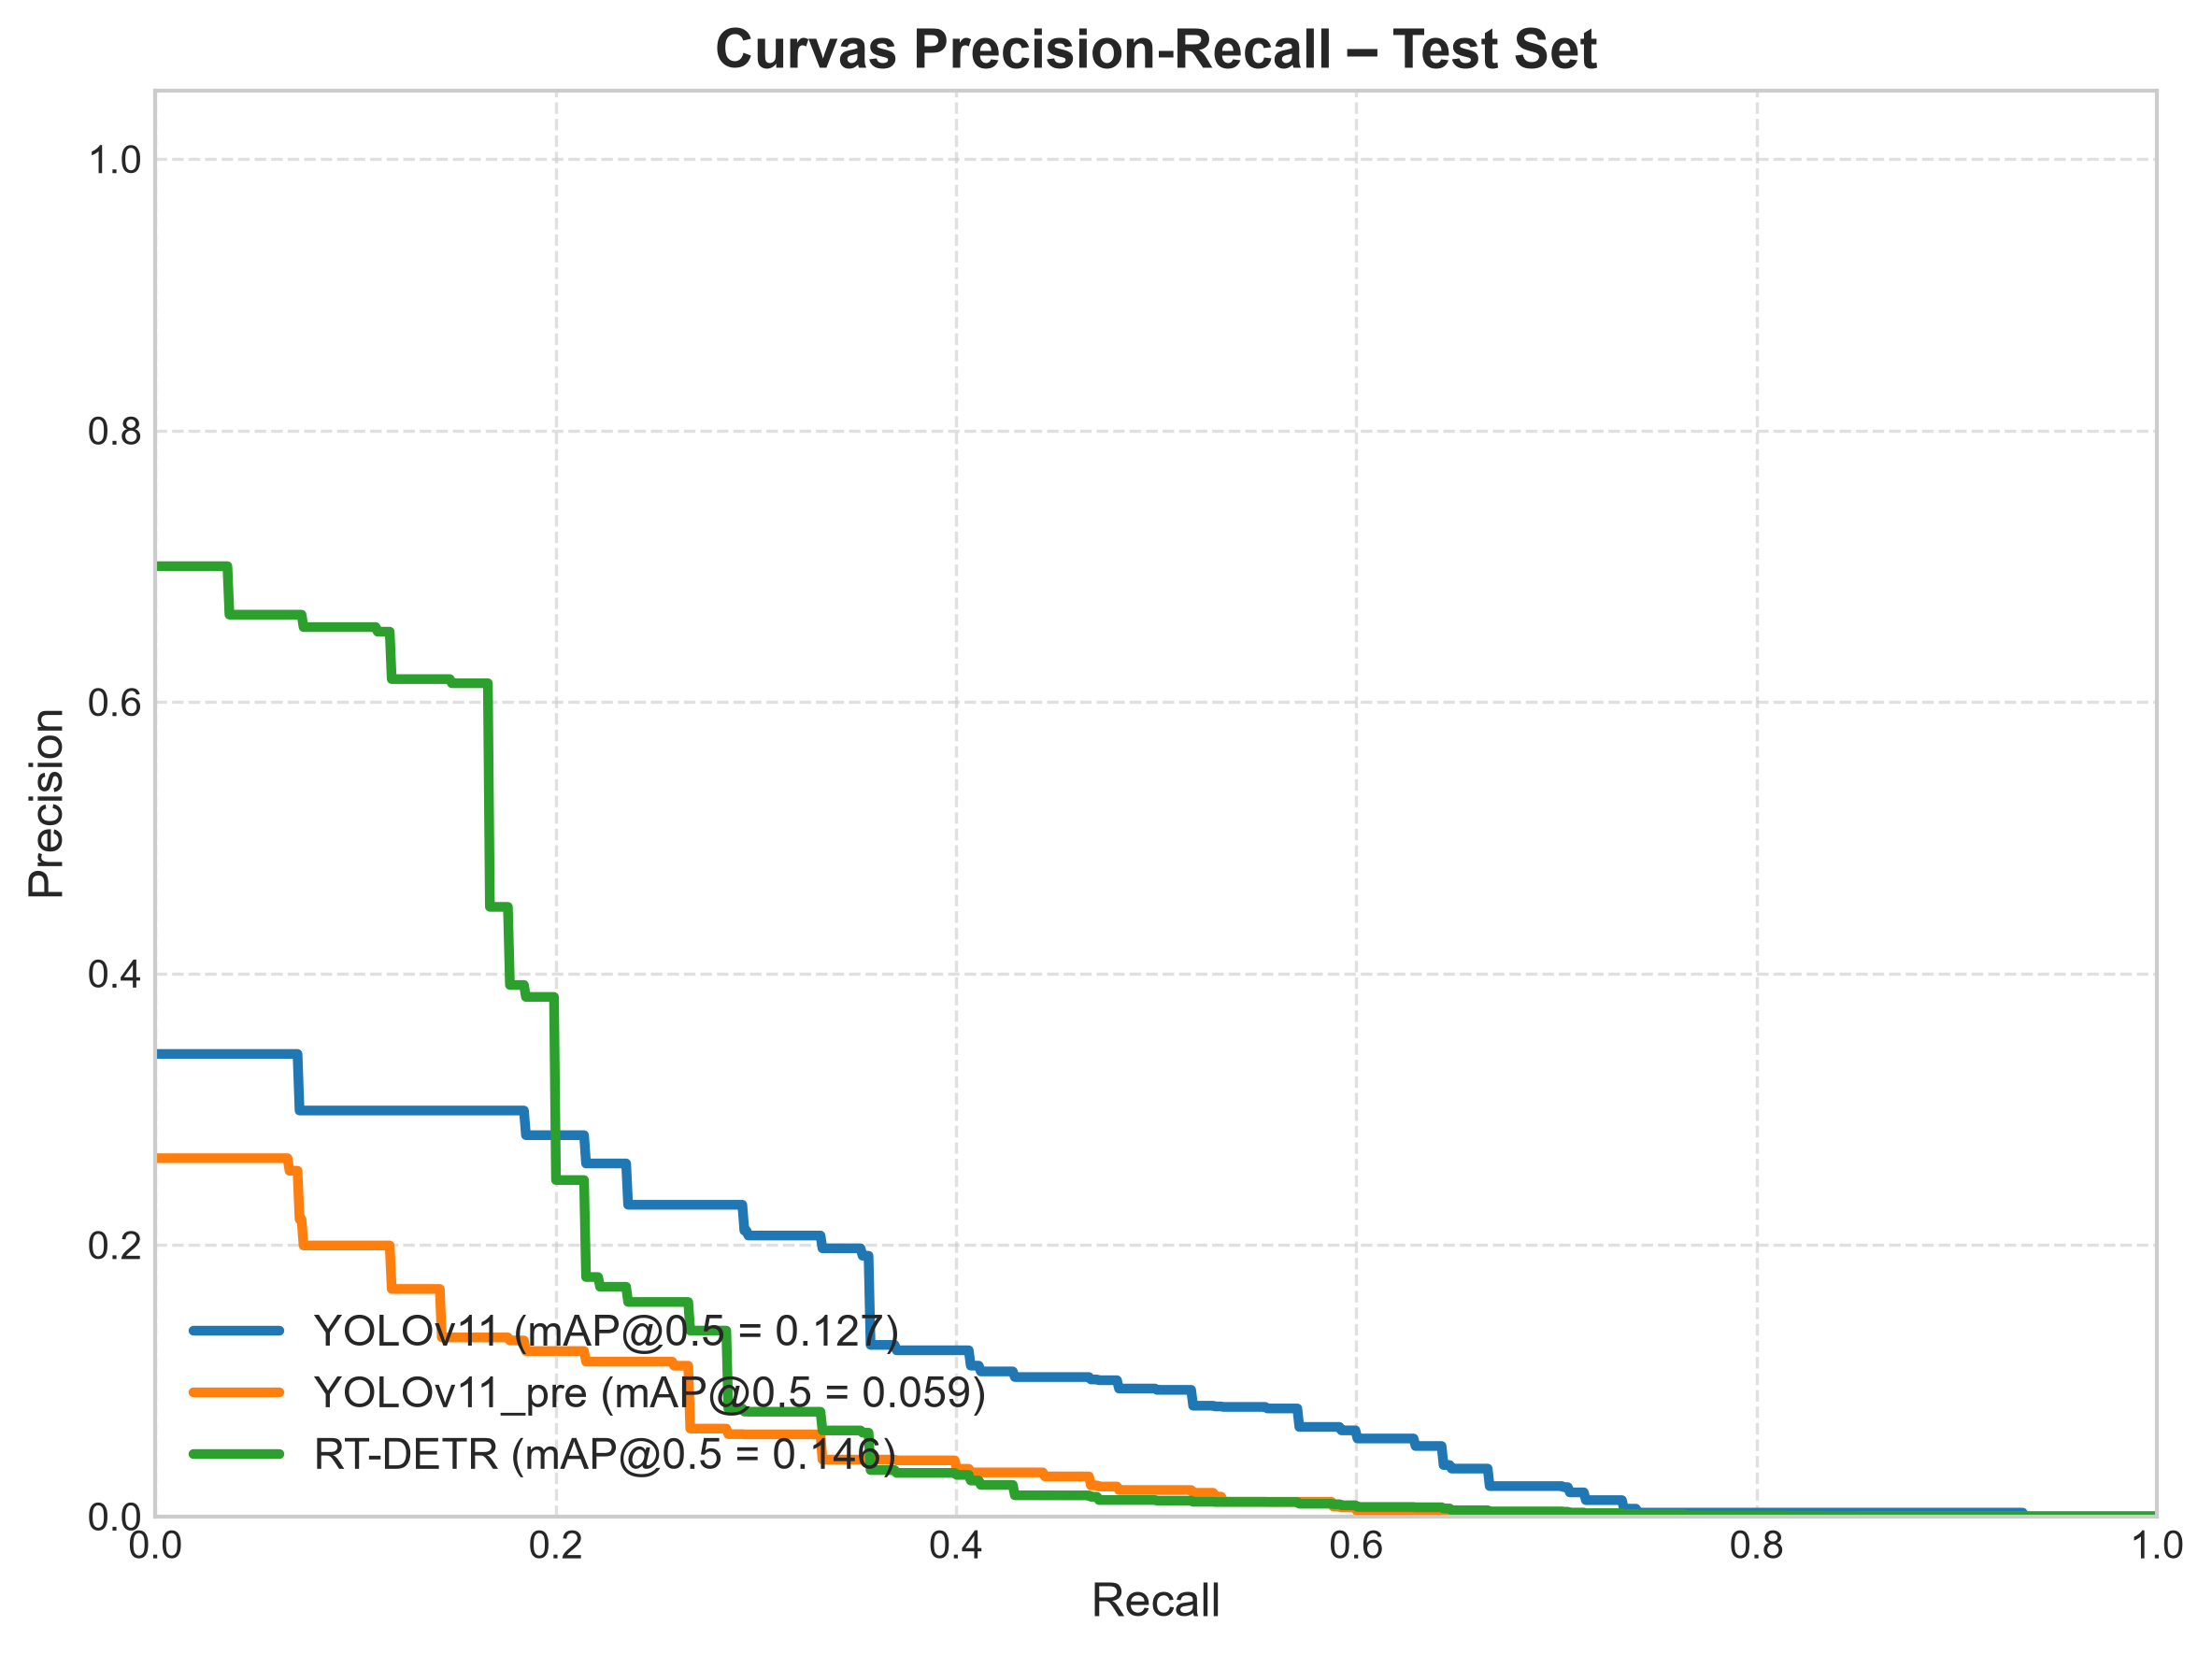
\includegraphics[width=0.9\linewidth]{04_pr_curves.png}
\caption{Curvas Precision-Recall de los tres modelos experimentales sobre el conjunto de Test. Se observa el severo decaimiento de confianza del bloque YOLO11m al aplicar preprocesamiento agresivo, en contraste con el equilibrio preservado de RT-DETR-L a lo largo del espectro evaluativo.}
\label{fig:pr_curves}
\end{figure}

Las matrices de confusión normalizadas de la Figura~\ref{fig:cm} permiten complementar el análisis de las métricas globales, mostrando las clases en las que cada modelo presenta mayores dificultades.

\begin{figure}[htbp]
\centering
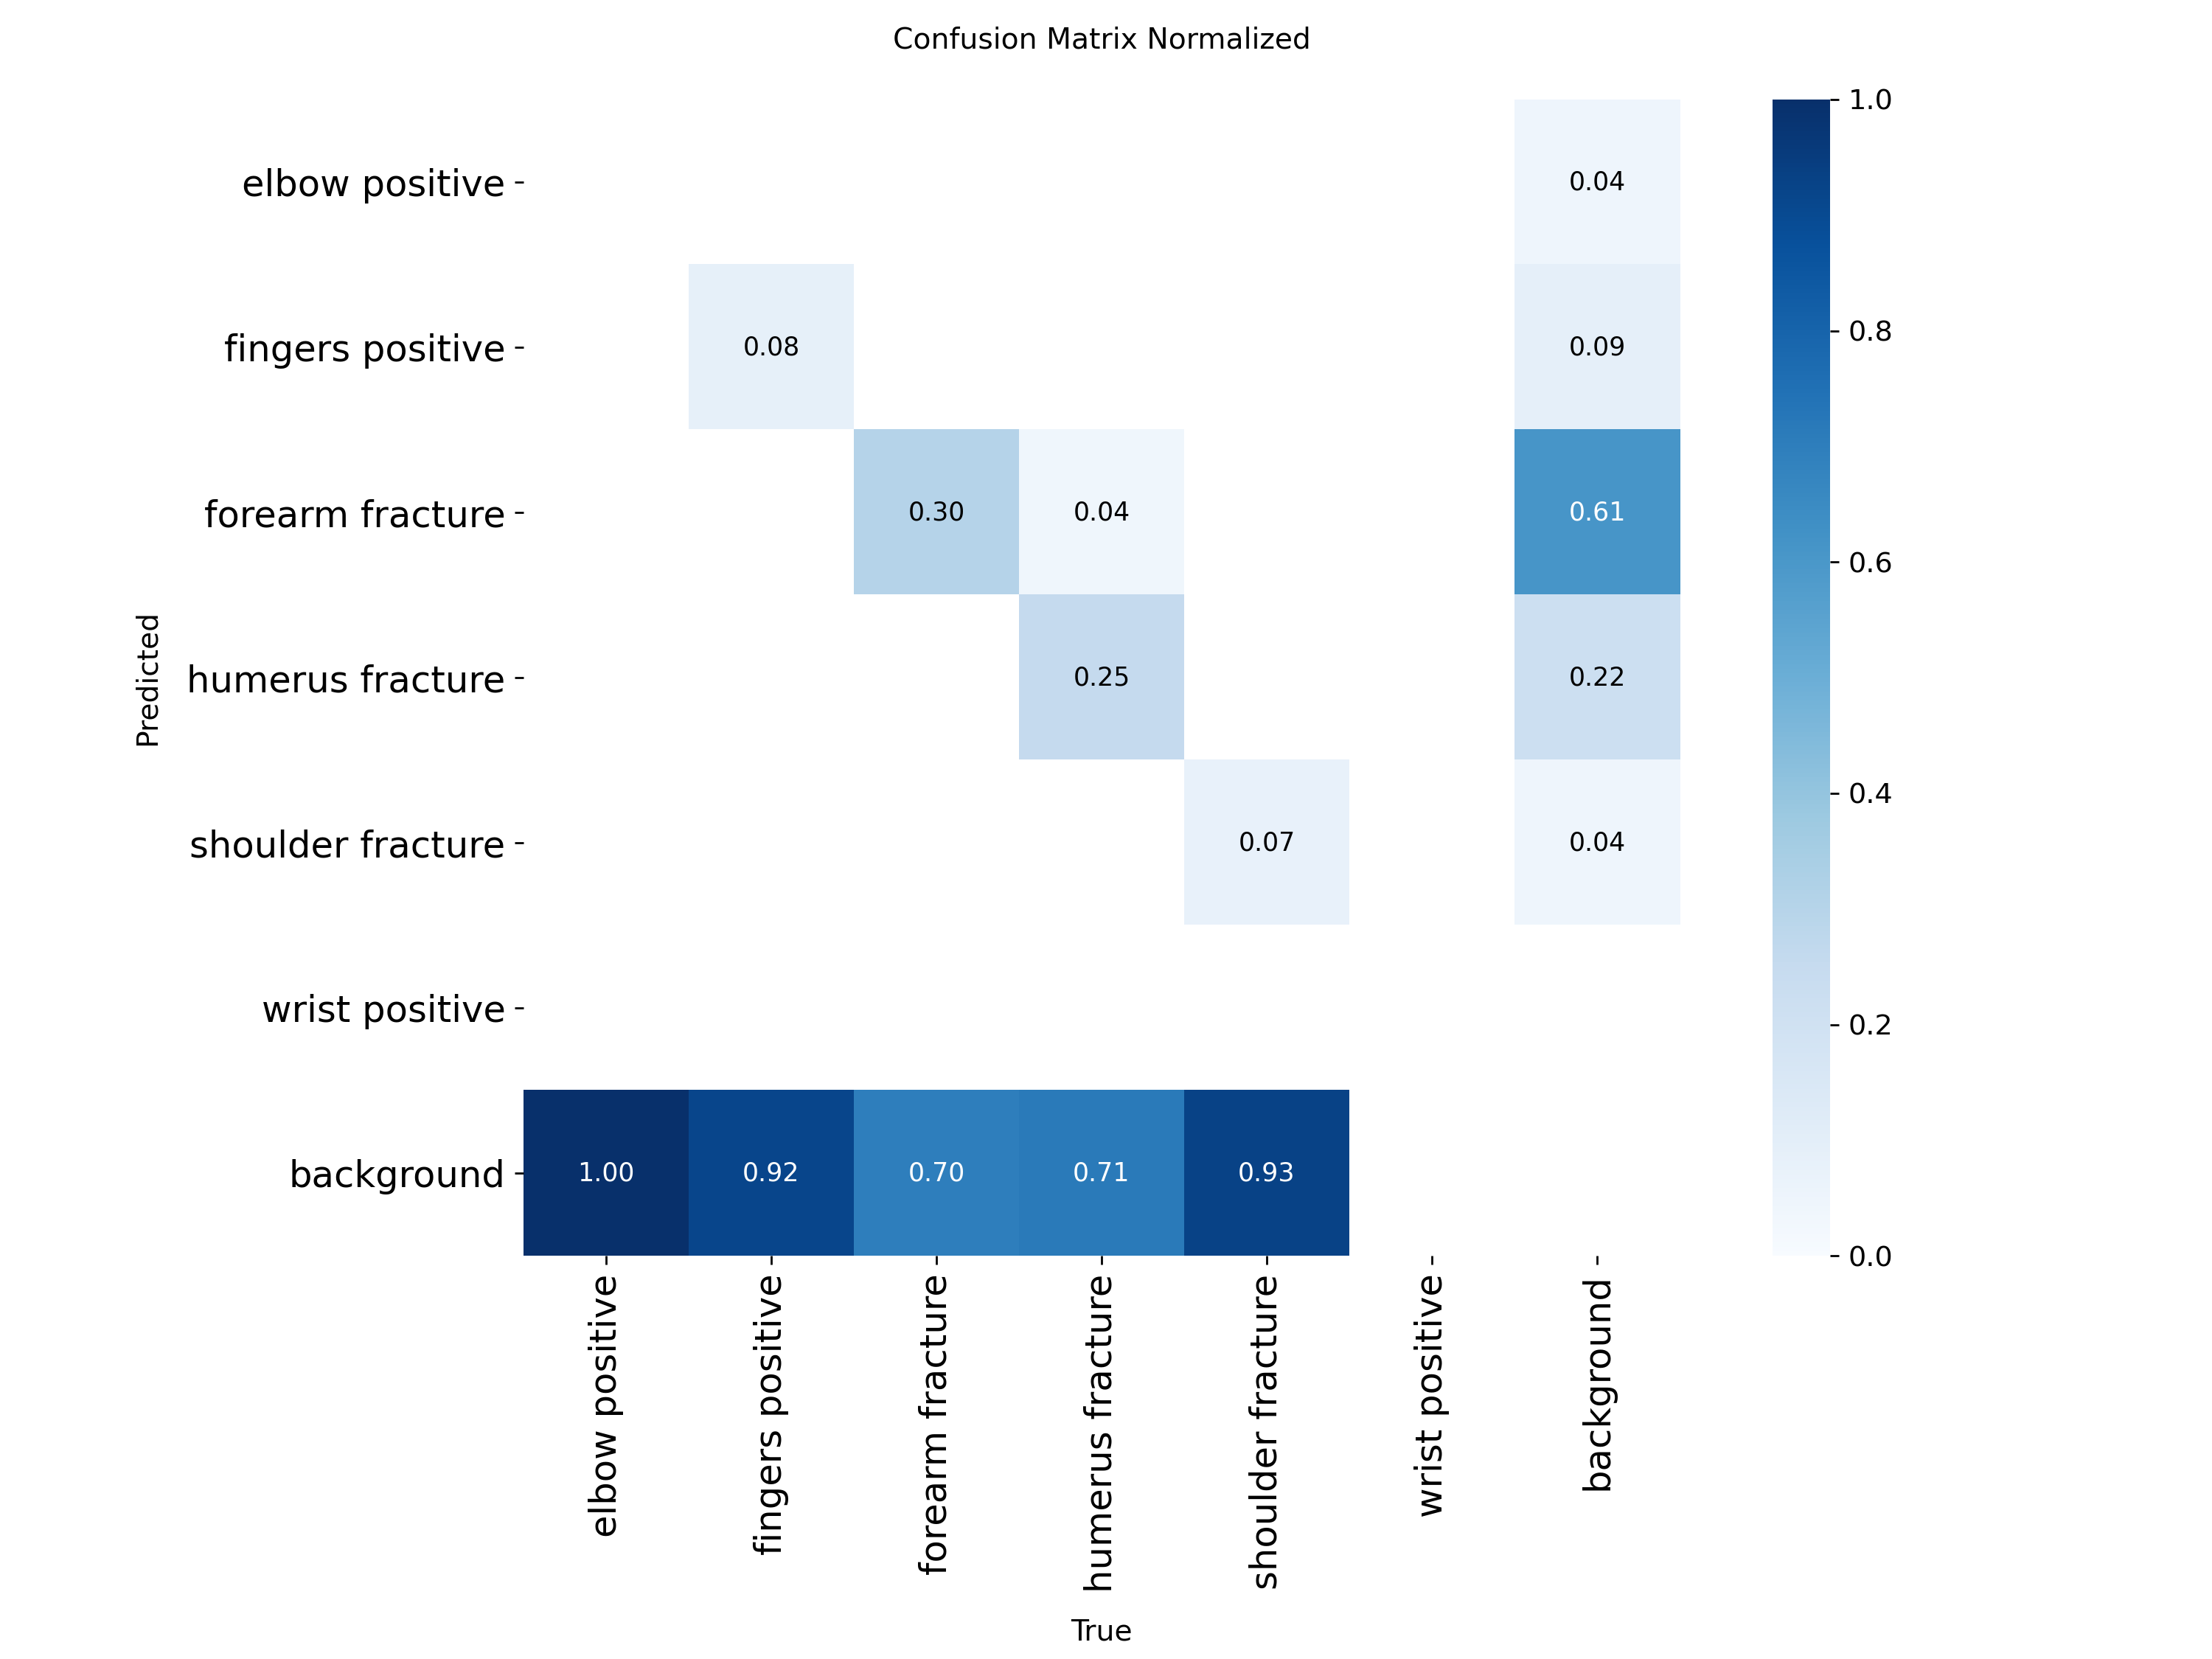
\includegraphics[width=0.9\linewidth]{yolo_confusion_matrix_normalized.png}
\vspace{0.2cm}

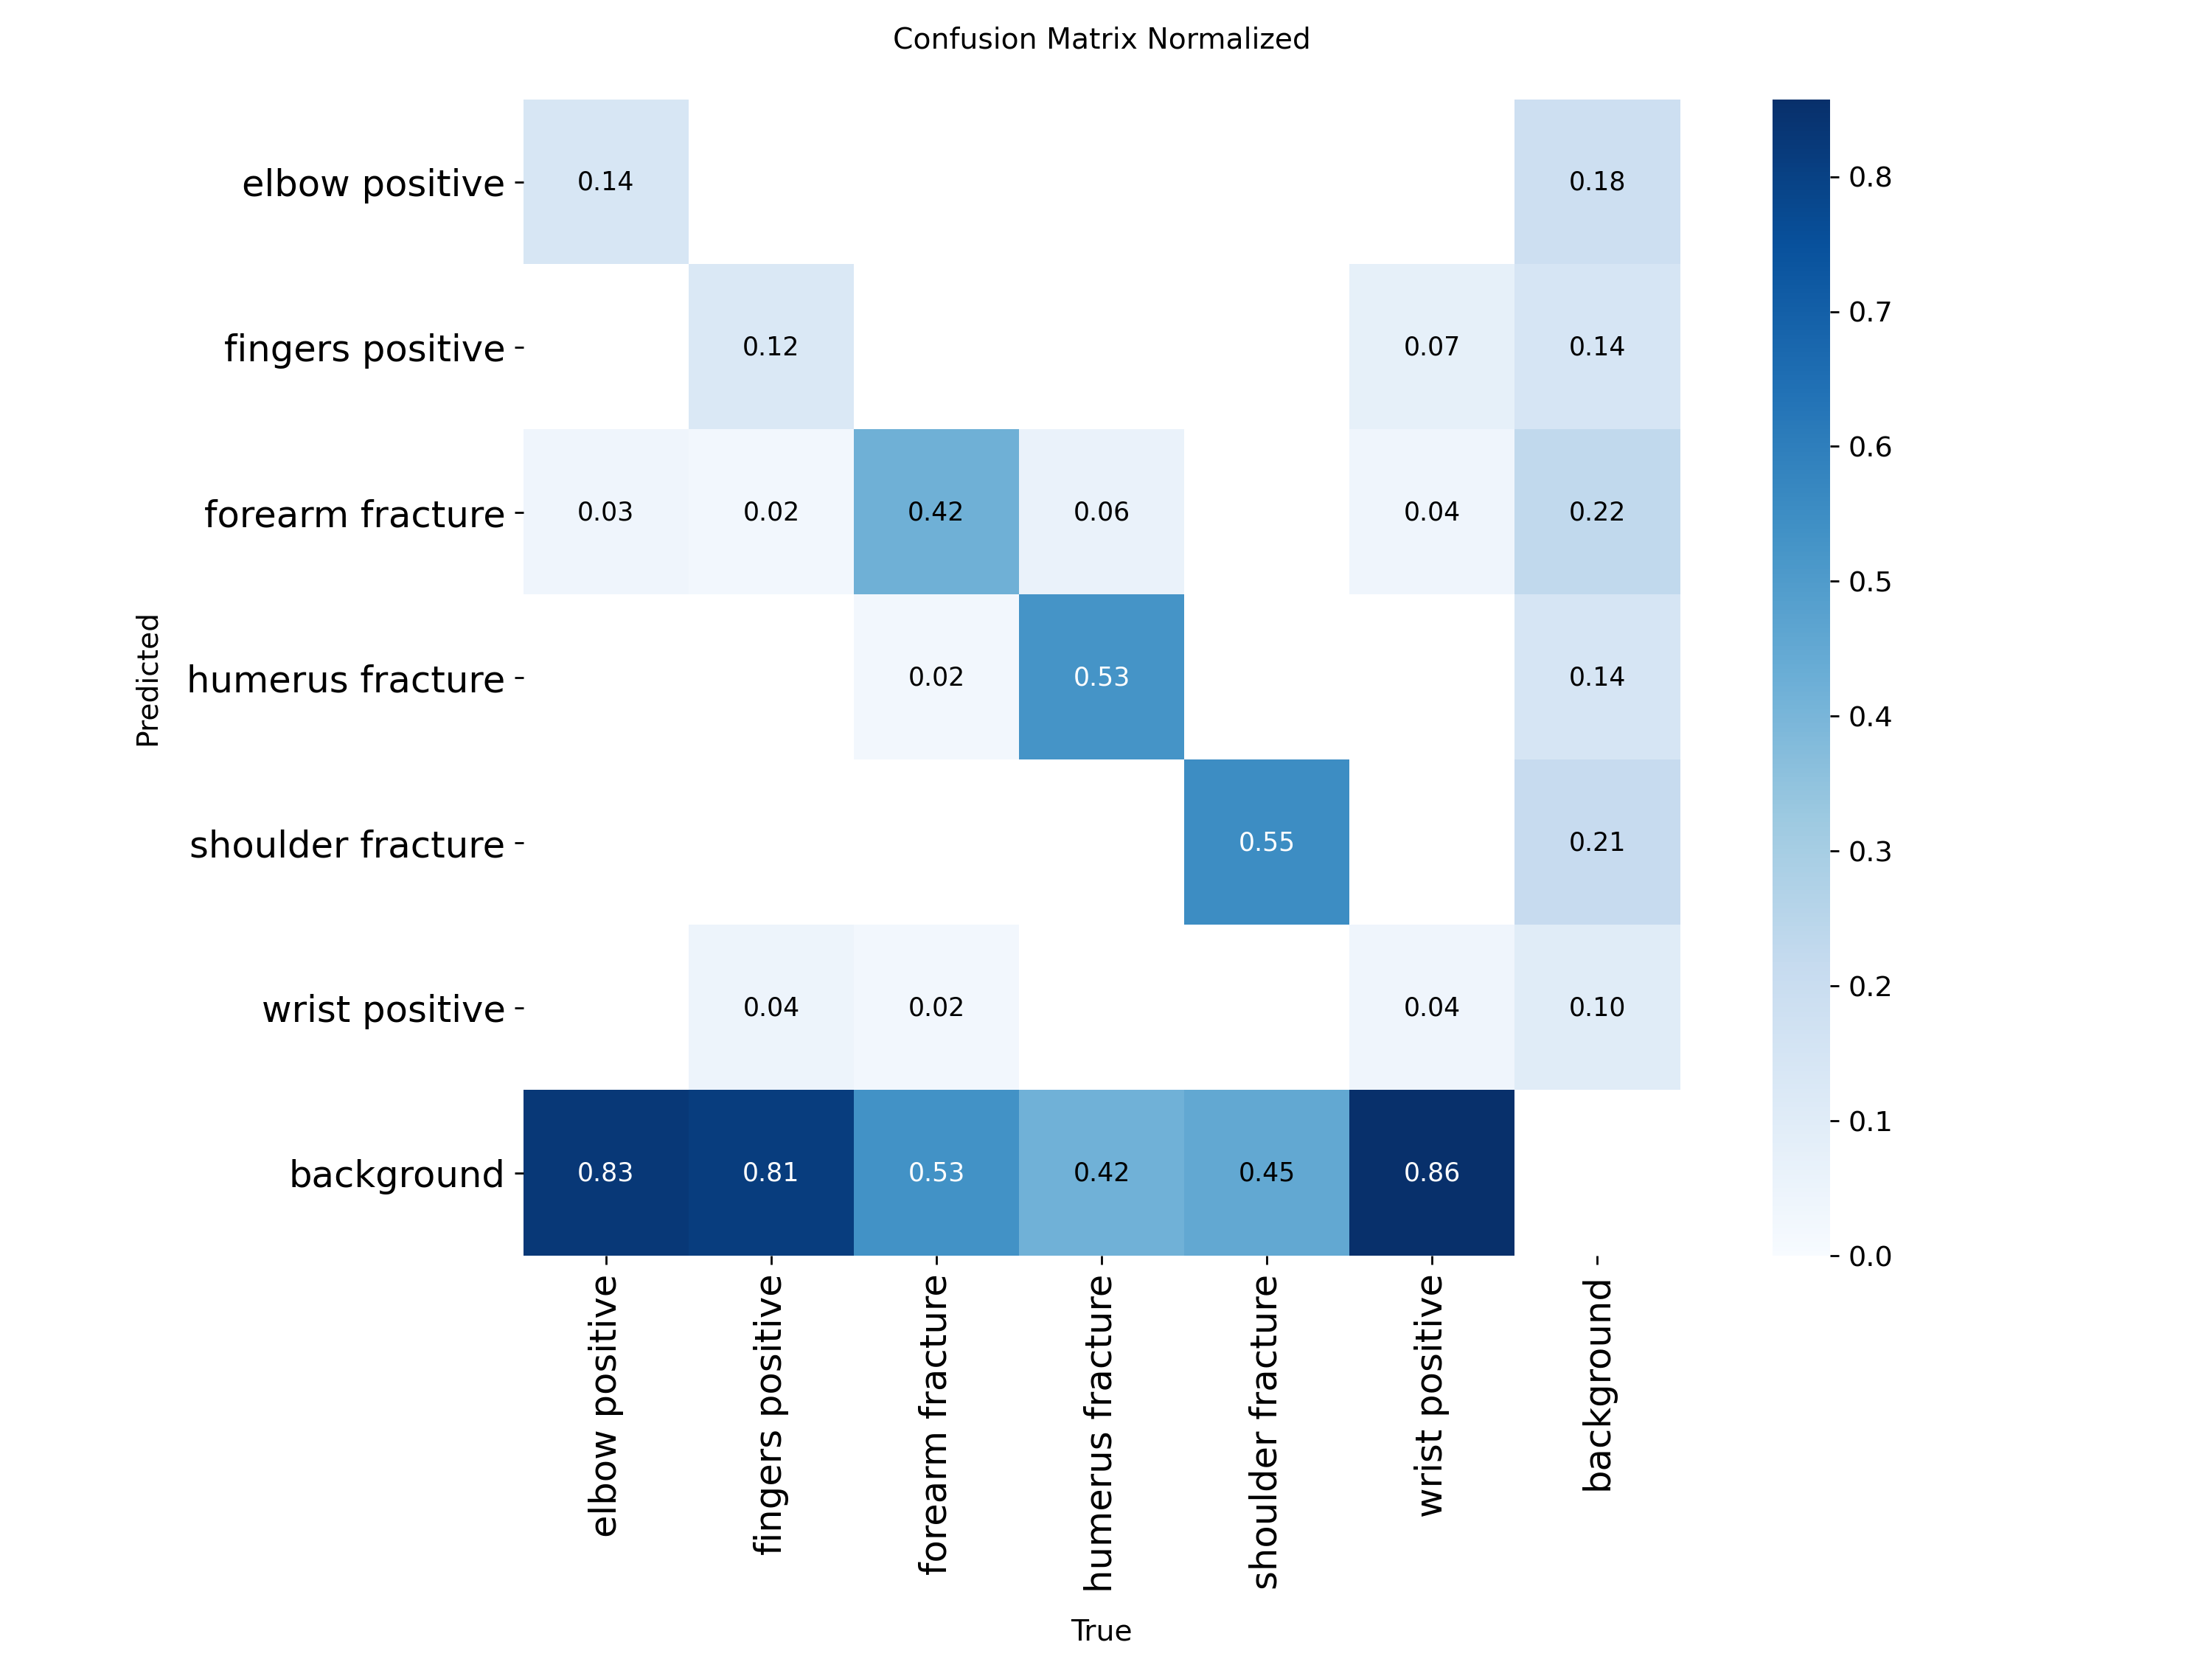
\includegraphics[width=0.9\linewidth]{rtdetr_confusion_matrix_normalized.png}
\caption{Matrices de confusión normalizadas. Arriba: YOLOv11m; Abajo: RT-DETR-L.}
\label{fig:cm}
\end{figure}

Finalmente, la Figura~\ref{fig:preds} presenta ejemplos cualitativos de las predicciones obtenidas. Esta comparación permite observar visualmente las diferencias entre las detecciones producidas por ambos modelos y complementar las métricas cuantitativas.

\begin{figure}[htbp]
\centering
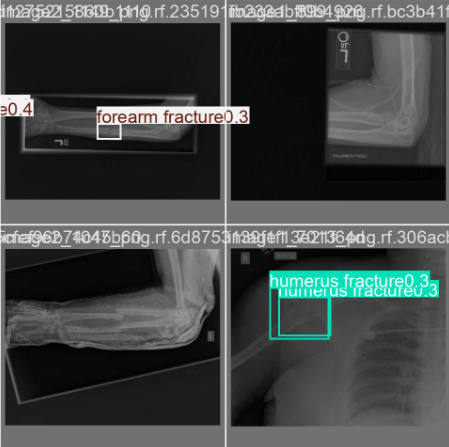
\includegraphics[width=0.9\linewidth]{yolo_pred_1.png}
\vspace{0.2cm}

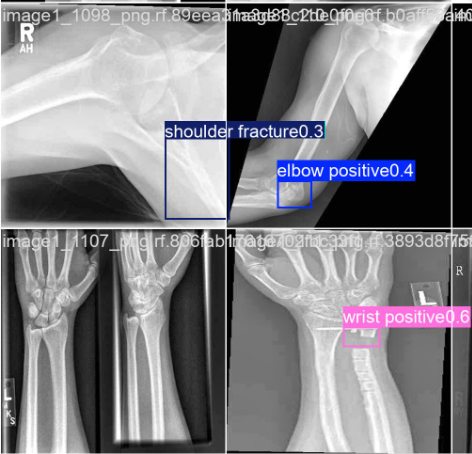
\includegraphics[width=0.9\linewidth]{rtdetr_Pred.png}
\caption{Comparativa cualitativa de predicciones. Arriba: YOLOv11m; Abajo: RT-DETR-L.}
\label{fig:preds}
\end{figure}


\subsection{Discusión de los resultados}

El primer experimento buscó responder si YOLO11 podía obtener un desempeño competitivo utilizando directamente las imágenes RAW. El resultado de mAP@0.5 de 0,2550 constituye la referencia experimental obtenida por nuestro modelo bajo esta condición. La drástica brecha frente al mAP@0.5 de 0,961 reportado por Srinivasu \textit{et al.} sobre este mismo conjunto de prueba invita fuertemente a considerar la presencia no documentada de fuga de datos (\textit{data leakage}) durante sus pasos globales de preservación y aumentos pre-procesados; contrariamente, el particionamiento estrictamente aislado empleado a lo largo del presente estudio arroja umbrales de detección y límite significativamente más realistas para un escenario clínico en donde las radiografías independientes de las patologías son mutuamente excluyentes. No obstante, subsiste como un hecho de relevancia que YOLO11m pueda capturar los mapas basales sin depender de adaptables fotométricos agresivos.

El segundo experimento permitió analizar una cuestión diferente: si el preprocesamiento que resultó beneficioso para YOLOv10 mantiene el mismo efecto sobre YOLO11. En este caso, el resultado fue contrario al esperado. El mAP@0.5 descendió de 0,2550 a 0,0766 y el F1-score alcanzó 0,1225. Por lo tanto, bajo las condiciones evaluadas, el preprocesamiento no produjo una mejora sobre YOLO11.

Este resultado no implica que CLAHE o \textit{unsharp masking} sean técnicas inadecuadas para imágenes radiográficas en general. Más bien, muestra que su efectividad depende de la interacción entre las transformaciones aplicadas, las características del dataset y la arquitectura utilizada. En consecuencia, la mejora observada previamente con YOLOv10 no puede asumirse como una propiedad general del dataset.

El tercer experimento incorporó RT-DETR-L sobre las imágenes preprocesadas. El modelo obtuvo un F1-score de 0,2854 y un mAP@0.5 de 0,2475, valores similares en mAP al resultado de YOLO11 sobre imágenes RAW, aunque con una latencia considerablemente mayor. Esta comparación debe interpretarse como exploratoria, ya que los dos modelos no fueron evaluados bajo exactamente las mismas condiciones de entrada.

La diferencia de latencia también resulta concluyente en relación de la profundidad arquitectónica. Evaluados bajo condiciones locales de inferencia (CPU), YOLO11m sobre imágenes originales presentó 512,3~ms por imagen frente a los 488,0~ms equivalentes en su versión preprocesada, mientras que RT-DETR-L presentó 1213,1~ms bajo las mismas condiciones evaluativas. Por lo tanto, el transformador exige aproximadamente 2,5 veces más tiempo subyacente que el pasaje convolucional unidimensional. Si bien se trata de un encarecimiento absoluto, frente a una guardia o sala de triage médico regular, un costo computacional final estipulado en $\approx 1$,25 segundos por radiografía no compromete negativamente el ciclo clínico, por lo que su adopción debe dictaminarse sobre la certidumbre ganada (F1-Score) de RT-DETR-L frente a la latencia minimizada de los detectores en tiempo real.


% ─── IV. CONCLUSIONES ─────────────────────────────────────────────────────────

\section{Conclusiones}

A partir de los experimentos realizados pueden establecerse las siguientes conclusiones:

\begin{enumerate}

    \item \textbf{YOLO11 sobre imágenes RAW presentó un desempeño limitado.}
    El modelo alcanzó un mAP@0.5 de 0,2550, valor considerablemente inferior al reportado para YOLOv10 sobre el mismo dataset. Por lo tanto, los resultados obtenidos no permiten sostener que YOLO11 pueda prescindir del preprocesamiento manteniendo un desempeño competitivo.

    \item \textbf{El preprocesamiento utilizado como referencia no produjo una mejora en YOLO11.}
    La aplicación de CLAHE y \textit{unsharp masking} redujo el mAP@0.5 de 0,2550 a 0,0766 y produjo un F1-score de 0,1225. Este resultado contrasta con la mejora reportada previamente para YOLOv10 sobre el mismo dataset \cite{b3_srinivasu}, mostrando que el efecto del preprocesamiento no necesariamente se mantiene al cambiar la arquitectura.

    \item \textbf{El comportamiento frente al desbalance varía entre las clases.}
    Las diferencias en la cantidad de anotaciones, especialmente entre \texttt{fingers positive} y \texttt{wrist positive}, deben considerarse al interpretar las métricas globales. El desempeño reducido observado en algunas categorías no puede explicarse únicamente por la cantidad de muestras, lo que evidencia la necesidad de realizar análisis por clase.

    \item \textbf{RT-DETR-L presentó un desempeño competitivo en mAP, pero con un costo computacional mayor.}
    Sobre el conjunto preprocesado, RT-DETR-L alcanzó un mAP@0.5 de 0,2475 y un F1-score de 0,2854, con una latencia de 41,68 ms por imagen. Esta latencia fue aproximadamente cuatro veces superior a la observada para YOLO11m.

    \item \textbf{La arquitectura y la preparación de los datos deben analizarse conjuntamente.}
    Los resultados muestran que una técnica de preprocesamiento que produjo mejoras en YOLOv10 no necesariamente genera el mismo efecto sobre YOLO11. Por lo tanto, la selección de un detector para radiografías no debería basarse únicamente en la arquitectura, sino también en la interacción entre el modelo y la representación de entrada.

\end{enumerate}

Como trabajo futuro se plantea ampliar el análisis mediante múltiples ejecuciones de cada configuración, ajustar sistemáticamente los hiperparámetros y evaluar estrategias específicas para las clases con menor cantidad de anotaciones. También sería conveniente incorporar métricas adicionales de localización y realizar un análisis más detallado de los falsos positivos y falsos negativos. Finalmente, cualquier consideración sobre utilización clínica requeriría validación sobre datasets externos y protocolos de evaluación independientes, por lo que los resultados obtenidos en este trabajo deben considerarse como una evaluación experimental de un prototipo y no como una validación clínica.


% ─── BIBLIOGRAFÍA ────────────────────────────────────────────────────────────

\begin{thebibliography}{00}

\bibitem{b1_srini}
S. A. Norris, D. Carrion, S. Uribe, and M. K. Badawy,
``Enhancing fracture detection in wrist radiographs via paired synthetic data generation,''
\textit{Scientific Reports (Monash Health)}, preprint, 2025.

\bibitem{b2_su}
Z. Su, et al.,
``Skeletal fracture detection with deep learning: A comprehensive review,''
\textit{Diagnostics}, vol. 13, no. 20, art. 3245, 2023.

\bibitem{b2_zebada}
A. M. Zebada and E. W. Pamungkas,
``Analysis of A Deep Learning Algorithm for Fracture Detection in X-Ray Images,''
\textit{International Journal of Advances in Data and Information Systems},
vol. 6, no. 3, pp. 716--734, 2025.

\bibitem{b3_srinivasu}
P. N. Srinivasu, et al.,
``Exploring the impact of hyperparameter and data augmentation in YOLO V10 for accurate bone fracture detection from X-ray images,''
\textit{Scientific Reports}, vol. 15, art. 9828, 2025.

\bibitem{b4_khan}
R. Khanam and M. Hussain,
``YOLOv11: An Overview of the Key Architectural Enhancements,''
\textit{arXiv preprint arXiv:2410.17725}, 2024.

\bibitem{b5_chen}
F. Chen, et al.,
``A Comparative Review of the Next-Generation YOLO Models: YOLOv10 and YOLO11,''
\textit{Journal of Computer Science and Artificial Intelligence},
vol. 3, no. 2, pp. 1--6, 2025.

\bibitem{b6_robo}
Roboflow Universe,
``Bone Fracture Detection Dataset,''
2024. [En línea]. Disponible:
https://universe.roboflow.com/veda/bone-fracture-detection-daoon

\bibitem{b7_leng}
Y. Zhao, et al.,
``DETRs Beat YOLOs on Real-time Object Detection,''
\textit{arXiv preprint arXiv:2304.08069}, 2023.

\end{thebibliography}

\end{document}